\section{Optical Tracking}
\subsection{Overview}
The Optical Tracking System is implemented with three subsystems:
\begin{enumerate}
  \item Video Extraction
  \item Pinhole Camera Model
  \item Epipolar Geometry
\end{enumerate}
\subsection{Video Extraction}
The Video Extraction system's function is to extract the location of a patricular object within the video footage. The objects, in this case, are differently colored small balls. The small balls represent sever key points of the Quadcopter. By determining the location of the balls, we will be able to calculate the position and attitude of the Quadcopter.
The procedure of video extraction is described as following:
\begin{enumerate}
  \item Shotting: Get images from camera,
  \item Transforming: transform the image to HSV colorspace,
  \item Extracting: use tresholding to extract pixels in patricular color range, then use histogram and backprojection to determin the probablity that the pixels belong to the model,
  \item Denoising: use opening and closing to denoise,
  \item Determining: use CamShift algorithm to determin the centroid of the extracted pixels.
\end{enumerate}
\subsubsection{Shooting}
In this project, v4l\footnote{a.k.a. Video For Linux} is as the middleware of OpenCV and camera. With \emph{v4l} and \emph{OpenCV}, reading an image from camera is as easy as following:
\lstset{language=python}
\begin{lstlisting}
cap = cv2.VideoCapture(source)
img = cap.read()
\end{lstlisting}
\subsubsection{Transforming}
Different from the RGB colorspace, HSV colorspace has a unique character: its V channel represents the brightness. If we remove V channel from tresholding, the same color profile will be able to work in different lighting conditions.
The transforming process is described below\cite{cite4}:
\begin{align}
  M &= \operatorname{max}(R, G, B) \\
  m &= \operatorname{min}(R, G, B) \\
  C &= M - m\\
  H^\prime &=
    \begin{cases}
      \mathrm{undefined},        &\mbox{if } C = 0 \\
      \frac{G - B}{C} \;\bmod 6, &\mbox{if } M = R \\
      \frac{B - R}{C} + 2,       &\mbox{if } M = G \\
      \frac{R - G}{C} + 4,       &\mbox{if } M = B
    \end{cases} \\
  H        &= 60^\circ \times H^\prime\\
  V &= M\\
   S &=
    \begin{cases}
      0,           &\mbox{if } C = 0 \\
      \frac{C}{V}, &\mbox{otherwise}
    \end{cases}
\end{align}
The code used to transform the image is:
\begin{lstlisting}
hsv = cv2.cvtColor(img, cv2.COLOR_BGR2HSV)
\end{lstlisting}
Note that by default, OpenCV uses BGR color space.
\subsubsection{Extracting}
OpenCV's built in treshold function is used to utilize multithreading.
The process of tresholding is printed below:
\begin{lstlisting}
mask = cv2.inRange(hsv, np.array((0., 60., 32.)), np.array((180., 255., 255.)))
\end{lstlisting}
However, simply tresholding is often not enough. The object tracked can have a complex color feature. In order to track the entire object, it is necessary to consider all of the features. Histogram is used to model the color distribution of an object, and me can then map the probability of pixels using backprojection.\\
\begin{figure}[h!]

  \centering
    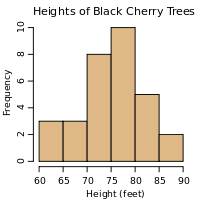
\includegraphics[width=0.2\textwidth]{../Pictures/histogram.JPG}
    \caption{A sample histogram\cite{cite5}}\\
\end{figure}
Backprojection uses the modeled histogram to find the probability that certain pixel belongs to the model. Consider an image matrix $M$, each pixel can be described as pair $(H_{i,j},S_{i,j})$. We can use the two values to create a 2D histogram that represents the distribution of certain color range in $H$ and $S$. Below is a sample 2D histogram generated by \emph{OpenCV Python Sample}.\\
\begin{figure}[h!]

  \centering
    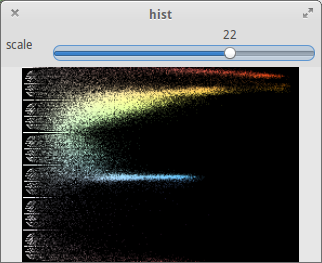
\includegraphics[width=0.3\textwidth]{../Pictures/2dhist.png}
    \caption{A sample 2D histogram}\\
\end{figure}
After generating the histogram, the probability that a pixel belongs to the model can be expressed by the following steps:
\begin{enumerate}
  \item Find the pair $(H_{i,j},S_{i,j})$ of a pixel,
  \item find the correspondent bin in the histogram,
  \item get the relative frequency of the bin.
\end{enumerate}
Then we can use the frequency to map a binary image. In this image, each pixel represents the probability that the correspondent pixel in the original image belongs to the model. Below is an example backproject image:\\
\begin{figure}[h!]

  \centering
    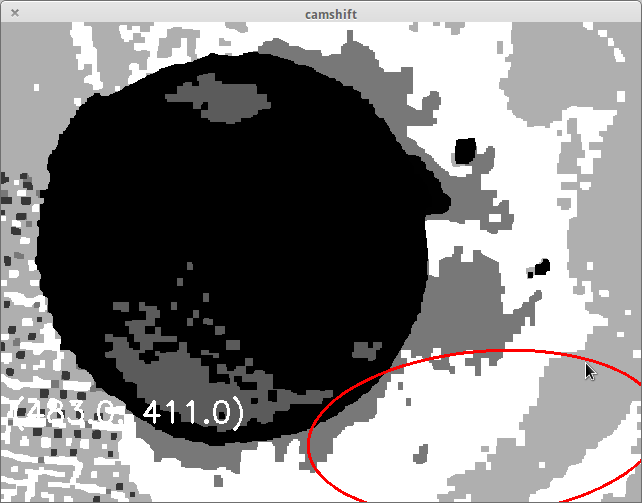
\includegraphics[width=0.5\textwidth]{../Pictures/backproject.png}
    \caption{A sample backprojrction}\\
\end{figure}
\subsubsection{Denoising}
After calculating the backproject image, we will be able to use morphology transformation to remove noises. In this projcet, we used Opening and Closing to remove small noise pixels and fill black pixel holes in the backprojection.\\
\begin{figure}[h!]

  \centering
    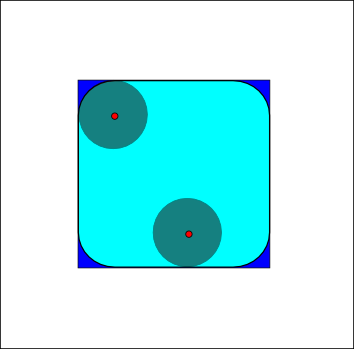
\includegraphics[width=0.3\textwidth]{../Pictures/Opening.png}
    \caption{Sample Opening operation\cite{cite7}}\\
\end{figure}
\begin{figure}[h!]

  \centering
    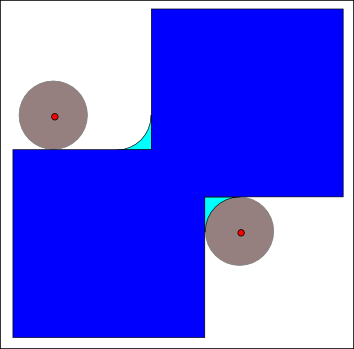
\includegraphics[width=0.3\textwidth]{../Pictures/Closing.png}
    \caption{Sample Closing operation\cite{cite6}}\\
\end{figure}

The result is significant. A great deal of noises is removed in this process:\\
\begin{figure}[h!]

  \centering
    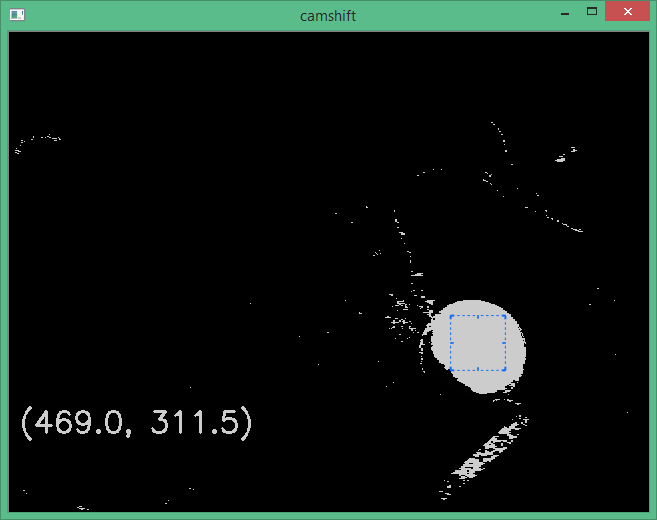
\includegraphics[width=0.3\textwidth]{../Pictures/before.png}
    \caption{Befor morphology transformation}\\
\end{figure}
\begin{figure}[h!]

  \centering
    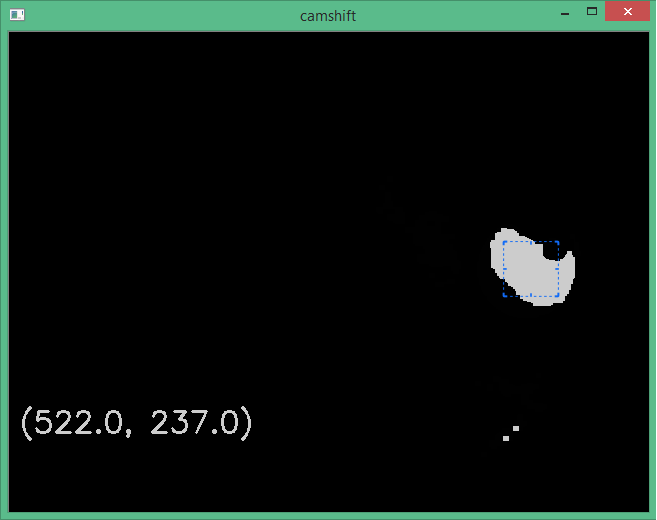
\includegraphics[width=0.3\textwidth]{../Pictures/after.png}
    \caption{After morphology transformation}\\
\end{figure}
